
%----------------------------------------------------------------------------------------
% Lecture 5: Introducing the Phillips Curve + Expected Inflation + Policy Rule (Whelan-style)
% - Keep output gap notation, connect once to unemployment (Okun)
% - Use clean TikZ figures (no external images)
% - SimpleDarkBlue theme, no heavy theorem boxes
%----------------------------------------------------------------------------------------

\documentclass[aspectratio=169,xcolor=dvipsnames]{beamer}
\usetheme{SimpleDarkBlue}

\usepackage{hyperref}
\usepackage{graphicx}
\usepackage{booktabs}
\usepackage{appendixnumberbeamer}
\usepackage{amsmath}
\usepackage{iftex}
\usepackage{tikz}
\usetikzlibrary{arrows.meta,calc}

% --- Font handling (compile anywhere) ---
\ifPDFTeX
  \usepackage[T1]{fontenc}
  \usepackage{lmodern}
  \usepackage{microtype}
\else
  \usepackage{fontspec}
  \usepackage{luatexja}
  \setmainfont{Alegreya Sans Light}[
    ItalicFont={* Italic},
    BoldFont={Alegreya Sans Medium},
    BoldItalicFont={Alegreya Sans Medium Italic}]
  \setsansfont{Alegreya Sans Light}[
    ItalicFont={* Italic},
    BoldFont={Alegreya Sans Medium},
    BoldItalicFont={Alegreya Sans Medium Italic}]
\fi

% ------------------------------------ %
% Section title page with Huge bf text %
% ------------------------------------ %
\AtBeginSection[]{
  \begin{frame}[noframenumbering, plain]
    \Huge{\centerline{\textbf{\insertsection}}}
  \end{frame}
}

%%% automatically add spaces into enumerate and itemize environment
\let\tempone\itemize
\let\temptwo\enditemize
\renewenvironment{itemize}{\tempone\addtolength{\itemsep}{\fill}}{\temptwo}
\let\tempa\enumerate
\let\tempb\endenumerate
\renewenvironment{enumerate}{\tempa\addtolength{\itemsep}{\fill}}{\tempb}

%%=============================================================
%%  FOOTLINE TEMPLATE
%%=============================================================
\defbeamertemplate*{footline}{shadow theme}{%
    \leavevmode\hbox{%
        \hypersetup{linkcolor=white,urlcolor=white,citecolor=white}
        \begin{beamercolorbox}[wd=1.02\paperwidth, ht=2.5ex, dp=1.125ex,
          leftskip=.3cm plus1fil, rightskip=0.3cm]{author in head/foot}%
            \insertsectionnavigationhorizontal{.80\textwidth}{}{} \hspace{.3cm}
            \hfill \#\ \insertframenumber \ / \ \inserttotalframenumber%
        \end{beamercolorbox}%
    }%
}
\setbeamertemplate{footline}[shadow theme]

%----------------------------------------------------------------------------------------
%    TITLE PAGE
%----------------------------------------------------------------------------------------
\title[Phillips Curve \& Policy]{Macroeconomics II (Spring 2026)\\\vspace{4pt}Lecture 5: Phillips Curve, Expected Inflation, and Monetary Policy}
\author[Hui-Jun Chen]{Hui-Jun Chen}
\institute[]{National Tsing Hua University}
\date{}

% --- TikZ styles (Whelan-like: clean axes, thick black lines, minimal decoration) ---
\tikzset{
  axis/.style={->,thick},
  curve/.style={thick},
  dashedcurve/.style={thick,dashed},
  lab/.style={fill=white,inner sep=1.3pt,font=\small},
  dot/.style={circle,fill=black,inner sep=1.4pt},
  >={Latex[length=3mm]}
}

\newcommand{\axesXY}[4]{%
  % xmin xmax ymin ymax are assumed by caller
  \draw[axis] (#1,0) -- (#2,0);
  \draw[axis] (0,#3) -- (0,#4);
}

\newcommand{\axeslabels}[2]{%
  \node[below right] at (2.65,0) {#1};
  \node[above left] at (0,3.85) {#2};
}

\begin{document}

%------------------------------------------------
\begin{frame}[plain,noframenumbering]
    \titlepage
\end{frame}

%------------------------------------------------
\section{From AD--AS to inflation dynamics}

%------------------------------------------------
\begin{frame}{Where we are after Lectures 3--4}
\begin{itemize}
\item Lecture 3 (figures): AD--AS explains \emph{direction} of $(Y,P)$ after shocks.
\item Lecture 4 (math): IS--LM / IS--MP gives AD as an equation and clarifies what shifts it.
\item Missing piece: a relationship that links \textbf{slack} to \textbf{inflation changes over time}.
\end{itemize}
\end{frame}

%------------------------------------------------
\begin{frame}{Two objects we keep using}
\begin{itemize}
\item Output gap: $x_t \equiv y_t-y_t^{FE}$.
\item Inflation: $\pi_t \equiv p_t-p_{t-1}$.
\end{itemize}

\vspace{0.2em}
\[
u_t-u_t^n \approx -\gamma x_t
\qquad (\gamma>0)\quad\text{(Okun)}
\]

\begin{itemize}
\item We write equations in $x_t$ but often talk in terms of unemployment tightness.
\end{itemize}
\end{frame}

%------------------------------------------------
\section{Phillips curve: the basic idea}

%------------------------------------------------
\begin{frame}{The basic Phillips curve idea (in words)}
\begin{itemize}
\item Tight economy: high demand for labor $\Rightarrow$ wage growth $\uparrow$ $\Rightarrow$ price pressure $\uparrow$.
\item Slack economy: weak labor market $\Rightarrow$ wage growth $\downarrow$ $\Rightarrow$ inflation pressure $\downarrow$.
\end{itemize}

\begin{itemize}
\item A simple reduced-form statement:
\[
\pi_t \text{ is higher when } x_t \text{ is higher.}
\]
\end{itemize}
\end{frame}

%------------------------------------------------
\begin{frame}{A classic picture: inflation vs unemployment (stylized)}
\begin{columns}
\begin{column}{0.62\textwidth}
\centering
\begin{tikzpicture}[x=1.15cm,y=1.05cm]
  % axes: u-u^n on x, pi on y
  \draw[axis] (-2.7,0) -- (2.8,0) node[below right] {$u_t-u_t^n$ (unemployment gap)};
  \draw[axis] (0,-0.2) -- (0,4.0) node[above left] {$\pi_t$ (inflation)};

  % downward curve
  \draw[curve] (-2.3,3.5) .. controls (-1.0,2.6) and (1.0,1.2) .. (2.3,0.8);
  \node[lab] at (1.65,1.25) {``Phillips curve''};

  % mark a couple points
  \fill (-1.2,2.7) circle (2pt);
  \fill (1.3,1.25) circle (2pt);
\end{tikzpicture}
\end{column}
\begin{column}{0.38\textwidth}
\small
\begin{itemize}
\item When unemployment is below natural ($u<u^n$), inflation tends to be higher.
\item When unemployment is above natural ($u>u^n$), inflation tends to be lower.
\item With Okun’s law, this is the same as using the output gap $x_t$.
\end{itemize}
\end{column}
\end{columns}
\end{frame}

%------------------------------------------------
\begin{frame}{Why the original curve broke down: expected inflation}
\begin{itemize}
\item In the 1970s, many economies saw:
\begin{itemize}
\item high unemployment \emph{and} high inflation (stagflation),
\item persistent inflation that did not disappear quickly.
\end{itemize}
\item Interpretation: the inflation-unemployment relation shifts when expected inflation changes.
\end{itemize}
\end{frame}

%------------------------------------------------
\section{Expectations-augmented Phillips curve}

%------------------------------------------------
\begin{frame}{Expectations-augmented Phillips curve (a useful form)}
\small
A common reduced form:
\[
\pi_t = \pi_t^e + \kappa x_t + u_t
\qquad (\kappa>0)
\]
\begin{itemize}
\item $\pi_t^e$: expected inflation (what wage/price setters build into contracts).
\item $\kappa x_t$: demand pressure via slack / tightness.
\item $u_t$: cost-push shock (energy, supply bottlenecks, markups).
\end{itemize}
\end{frame}

%------------------------------------------------
\begin{frame}{A picture in $(x,\pi)$ space: higher expected inflation shifts the curve up}
\begin{columns}
\begin{column}{0.62\textwidth}
\centering
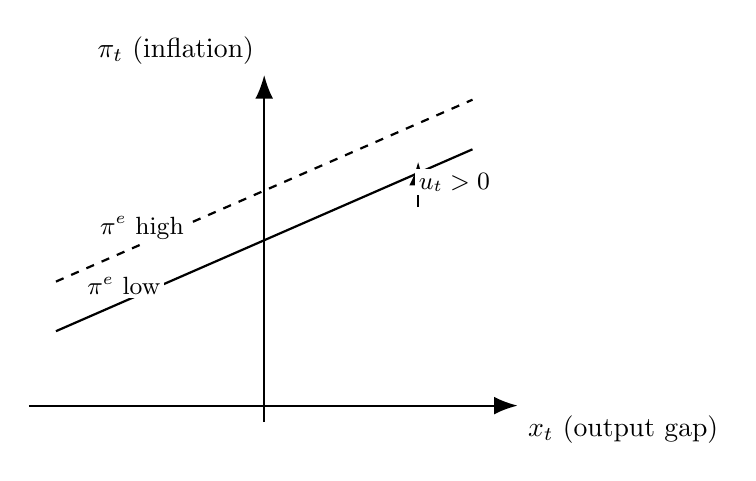
\begin{tikzpicture}[x=1.15cm,y=1.05cm]
  % axes
  \draw[axis] (-2.6,0) -- (2.8,0) node[below right] {$x_t$ (output gap)};
  \draw[axis] (0,-0.2) -- (0,4.0) node[above left] {$\pi_t$ (inflation)};

  % PC for low expected inflation
  \draw[curve] (-2.3,0.9) -- (2.3,3.1);
  \node[lab] at (-1.55,1.45) {$\pi^e$ low};

  % PC for high expected inflation (shift up)
  \draw[dashedcurve] (-2.3,1.5) -- (2.3,3.7);
  \node[lab] at (-1.35,2.15) {$\pi^e$ high};

  % cost-push shift arrow
  \draw[->,thick] (1.7,2.4) -- (1.7,2.95);
  \node[lab] at (2.1,2.70) {$u_t>0$};
\end{tikzpicture}
\end{column}
\begin{column}{0.38\textwidth}
\small
\begin{itemize}
\item Same $x_t$ can imply very different inflation if $\pi_t^e$ is different.
\item Cost-push shocks also shift inflation upward for a given $x_t$.
\end{itemize}
\end{column}
\end{columns}
\end{frame}

%------------------------------------------------
\begin{frame}{How to read the equation as a ``moving curve''}
\begin{itemize}
\item Fix expected inflation $\pi_t^e$ and cost-push $u_t$:
\[
\pi_t = \underbrace{\pi_t^e+u_t}_{\text{intercept}} + \kappa x_t.
\]
\item The slope $\kappa$ is the sensitivity of inflation to slack.
\item The intercept moves when:
\begin{itemize}
\item expected inflation changes ($\pi_t^e$),
\item cost-push shocks hit ($u_t$).
\end{itemize}
\end{itemize}
\end{frame}

%------------------------------------------------
\section{Expected inflation: what could $\pi_t^e$ mean?}

%------------------------------------------------
\begin{frame}{Two simple expectation rules (we will compare them later)}
\begin{enumerate}
\item \textbf{Adaptive / backward-looking:} $\pi_t^e=\pi_{t-1}$.
\item \textbf{Forward-looking:} $\pi_t^e=\mathbb{E}_t \pi_{t+1}$.
\end{enumerate}

\begin{itemize}
\item For now: treat $\pi_t^e$ as a \emph{state variable} that can drift or be anchored by policy.
\end{itemize}
\end{frame}

%------------------------------------------------
\begin{frame}{Anchored expectations (the key policy phrase)}
\begin{itemize}
\item ``Expectations are anchored'' means:
\begin{itemize}
\item long-run expected inflation stays near the target $\pi^\ast$,
\item temporary shocks do not shift $\pi^e$ much.
\end{itemize}
\item ``Unanchored'' means:
\begin{itemize}
\item inflation rises today and people start building that into wages/prices tomorrow,
\item Phillips curve shifts upward persistently.
\end{itemize}
\end{itemize}
\end{frame}

%------------------------------------------------
\section{Central bank practice: inflation targeting and Taylor rules}

%------------------------------------------------
\begin{frame}{A policy description students will see everywhere}
\small
Taylor-style reaction function:
\[
i_t = \bar i + \phi_\pi(\pi_t-\pi^\ast) + \phi_x x_t.
\]
\begin{itemize}
\item Inflation targeting: $\phi_\pi>0$ (lean against inflation deviations).
\item Output stabilization: $\phi_x>0$ (lean against overheating / slack).
\item ``Taylor principle'' language: often $\phi_\pi>1$ is emphasized once we add expectations formally.
\end{itemize}
\end{frame}

%------------------------------------------------
\begin{frame}{From policy rule to a downward AD in $(x,\pi)$ space (picture)}
\begin{columns}
\begin{column}{0.62\textwidth}
\centering
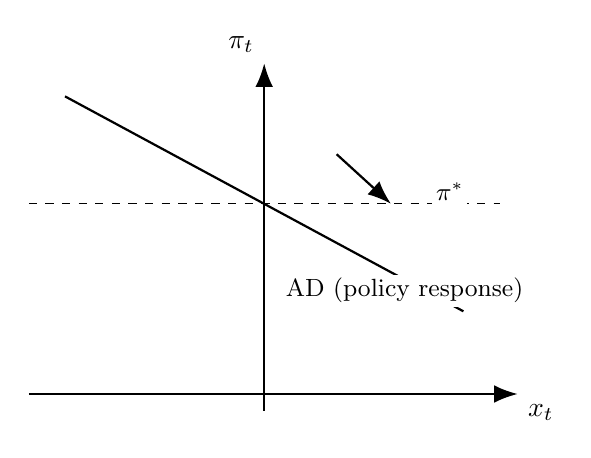
\begin{tikzpicture}[x=1.15cm,y=1.05cm]
  % axes
  \draw[axis] (-2.6,0) -- (2.8,0) node[below right] {$x_t$};
  \draw[axis] (0,-0.2) -- (0,4.0) node[above left] {$\pi_t$};

  % downward AD: x = xbar - eta(pi-pi*)
  \draw[curve] (-2.2,3.6) -- (2.2,1.0);
  \node[lab] at (1.55,1.25) {AD (policy response)};

  % mark target inflation line (horizontal)
  \draw[dashed] (-2.6,2.3) -- (2.6,2.3);
  \node[lab] at (2.05,2.45) {$\pi^\ast$};

  % arrow: higher pi -> lower x
  \draw[->,thick] (0.8,2.9) -- (1.4,2.3);
\end{tikzpicture}
\end{column}
\begin{column}{0.38\textwidth}
\small
\begin{itemize}
\item Higher inflation triggers tighter policy ($i_t\uparrow$).
\item Real rate rises (given expectations) $\Rightarrow$ demand cools $\Rightarrow$ $x_t$ falls.
\item This is the IS--MP view of AD in $(x,\pi)$ space.
\end{itemize}
\end{column}
\end{columns}
\end{frame}

%------------------------------------------------
\begin{frame}{Combine AD and Phillips curve (static intersection)}
\begin{columns}
\begin{column}{0.62\textwidth}
\centering
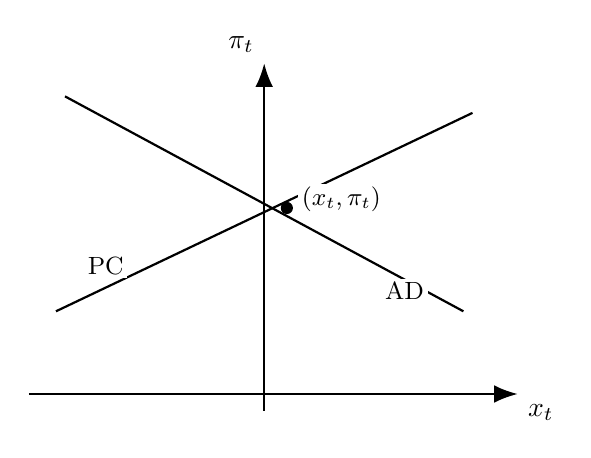
\begin{tikzpicture}[x=1.15cm,y=1.05cm]
  % axes
  \draw[axis] (-2.6,0) -- (2.8,0) node[below right] {$x_t$};
  \draw[axis] (0,-0.2) -- (0,4.0) node[above left] {$\pi_t$};

  % AD
  \draw[curve] (-2.2,3.6) -- (2.2,1.0);
  \node[lab] at (1.55,1.25) {AD};

  % PC
  \draw[curve] (-2.3,1.0) -- (2.3,3.4);
  \node[lab] at (-1.75,1.55) {PC};

  % intersection
  \coordinate (E) at (0.25,2.25);
  \fill (E) circle (2.2pt);
  \node[lab,anchor=west] at ($(E)+(0.12,0.10)$) {$(x_t,\pi_t)$};
\end{tikzpicture}
\end{column}
\begin{column}{0.38\textwidth}
\small
\begin{itemize}
\item AD pins $x$ as a function of inflation (policy).
\item PC pins inflation as a function of $x$ (price setting / marginal cost).
\item Their intersection is the one-period outcome.
\end{itemize}
\end{column}
\end{columns}
\end{frame}

%------------------------------------------------
\section{Reading shocks with the new language}

%------------------------------------------------
\begin{frame}{Demand shock: shifts AD}
\begin{columns}
\begin{column}{0.62\textwidth}
\centering
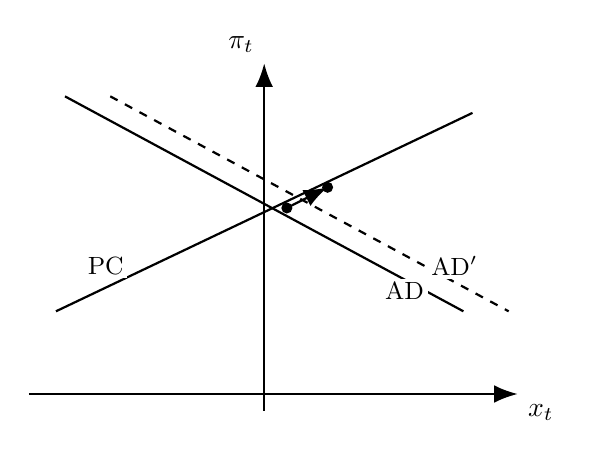
\begin{tikzpicture}[x=1.15cm,y=1.05cm]
  % axes
  \draw[axis] (-2.6,0) -- (2.8,0) node[below right] {$x_t$};
  \draw[axis] (0,-0.2) -- (0,4.0) node[above left] {$\pi_t$};

  % PC fixed
  \draw[curve] (-2.3,1.0) -- (2.3,3.4);
  \node[lab] at (-1.75,1.55) {PC};

  % AD baseline
  \draw[curve] (-2.2,3.6) -- (2.2,1.0);
  \node[lab] at (1.55,1.25) {AD};

  % AD' right
  \draw[dashedcurve] (-1.7,3.6) -- (2.7,1.0);
  \node[lab] at (2.1,1.55) {AD$'$};

  % intersections
  \coordinate (E0) at (0.25,2.25);
  \fill (E0) circle (2.0pt);
  \coordinate (E1) at (0.70,2.50);
  \fill (E1) circle (2.0pt);
  \draw[->,thick] (E0) -- (E1);
\end{tikzpicture}
\end{column}
\begin{column}{0.38\textwidth}
\small
\begin{itemize}
\item Examples: fiscal expansion, credit loosening, optimism.
\item Outcome: $x_t\uparrow$ and $\pi_t\uparrow$ (demand-driven inflation).
\end{itemize}
\end{column}
\end{columns}
\end{frame}

%------------------------------------------------
\begin{frame}{Cost-push shock: shifts Phillips curve}
\begin{columns}
\begin{column}{0.62\textwidth}
\centering
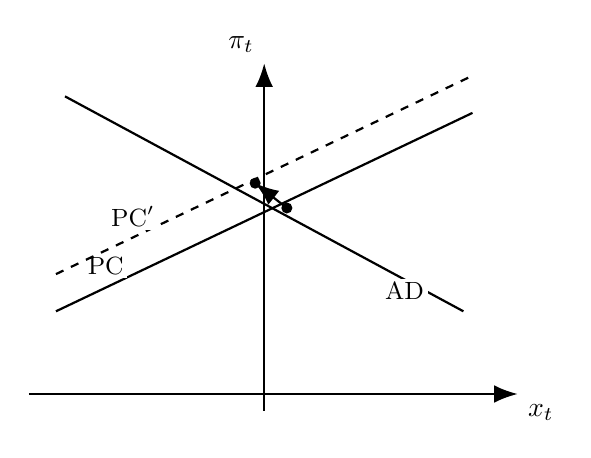
\begin{tikzpicture}[x=1.15cm,y=1.05cm]
  % axes
  \draw[axis] (-2.6,0) -- (2.8,0) node[below right] {$x_t$};
  \draw[axis] (0,-0.2) -- (0,4.0) node[above left] {$\pi_t$};

  % AD fixed
  \draw[curve] (-2.2,3.6) -- (2.2,1.0);
  \node[lab] at (1.55,1.25) {AD};

  % PC baseline
  \draw[curve] (-2.3,1.0) -- (2.3,3.4);
  \node[lab] at (-1.75,1.55) {PC};

  % PC' up
  \draw[dashedcurve] (-2.3,1.45) -- (2.3,3.85);
  \node[lab] at (-1.45,2.15) {PC$'$};

  % intersections
  \coordinate (E0) at (0.25,2.25);
  \fill (E0) circle (2.0pt);
  \coordinate (E1) at (-0.10,2.55);
  \fill (E1) circle (2.0pt);
  \draw[->,thick] (E0) -- (E1);
\end{tikzpicture}
\end{column}
\begin{column}{0.38\textwidth}
\small
\begin{itemize}
\item Examples: energy shock, bottlenecks, markup shock.
\item Outcome: $\pi_t\uparrow$ while $x_t$ weakens (stagflation pressure).
\end{itemize}
\end{column}
\end{columns}
\end{frame}

%------------------------------------------------
\section{Where Lecture 6 starts (Old Keynesian in detail)}

%------------------------------------------------
\begin{frame}{What we did today (without committing to a full dynamic model)}
\begin{itemize}
\item Phillips curve: $\pi_t=\pi_t^e+\kappa x_t+u_t$.
\item Policy rule: $i_t=\bar i+\phi_\pi(\pi_t-\pi^\ast)+\phi_x x_t$.
\item AD in $(x,\pi)$ space: higher inflation triggers tighter policy $\Rightarrow$ $x$ falls.
\end{itemize}
\end{frame}

%------------------------------------------------
\begin{frame}{Next time: a dynamic law of motion}
\begin{itemize}
\item Specify $\pi_t^e$ explicitly (e.g., adaptive: $\pi_t^e=\pi_{t-1}$).
\item Combine IS + rule + Phillips to get a time path for inflation.
\item That is the detailed Old Keynesian model (Lecture 6).
\end{itemize}
\end{frame}

\end{document}
